\documentclass[11pt,a4paper]{article}
\usepackage[margin=1in]{geometry}
\usepackage{enumitem}
\usepackage{amsmath}
\usepackage{graphicx}
\usepackage[colorlinks=true, allcolors=blue]{hyperref}
\usepackage{fancyhdr}
\usepackage[nottoc,numbib]{tocbibind}
\usepackage{indentfirst}
\usepackage{algpseudocode}

\pagestyle{fancy}
\setlength{\headheight}{14pt}
\linespread{1.8}
\let\oldheadrule\headrule
\renewcommand{\headrule}{\color{red}\oldheadrule}
\lhead{2023 MGCS 670 Revenue Management}
\rhead{Group Assignment 1}

\title{
\large{McGill University | Desautels Faculty of Management}\\
\hfill \break
\hfill \break
\hfill \break
\hfill \break
\\\Large MGSC 670 - Revenue Management\\
\textbf{Group Assignment 1: Markdown Strategy}\\
\hfill \break
\hfill \break
}

\author{\\\\
261083570 Konstantin Volodin\\
261078897 Ying-Fang Liang\\
260658030 Emery Dittmer\\
261077392 Julie Chanzy\\\\
\hfill \break
\\\\\textbf{Instructor:} Professor Maxime Cohen\\
\hfill \break
}

\date{\emph{May 2023}}

\begin{document}

\maketitle
\thispagestyle{empty}
\pagebreak

\tableofcontents
\pagenumbering{gobble}
\pagebreak

\pagenumbering{arabic}
\setcounter{page}{1}
\section{Introduction}
Any modern consumer recognizes words like “discount”, “clearance”, or “liquidation.” 
Behind the scenes of these words is a carefully orchestrated pricing and markdown strategy for each product from retailers. 
The relationship between price and demand is well documented by the field of economics. 
With perfect information and competition, as the price increases, the demand decreases, and vice-versa. 
Simplified price is, therefore, a control mechanism for the quantity of an item sold. 

Our report will examine and propose a markdown strategy for a hypothetical retail fashion company that sells goods to customers (B2C). 
Within this framework, the organization holds 2,000 units of inventory with a starting price of \$60. 
The inventory must be sold within 15 weeks. We have three discount options, hence a price that varies among: full price, -10\% -20\% and -40\% off. 
Each discount is irreversible. Each pricing strategy adopted will generate a unique demand curve. 
This inventory-to-price scenario is illustrated in USC Marshall’s School of Business retail game \cite{RetailerGame}. 
The web application simulates market behaviour based on a user-generated markdown strategy.\\

\begin{figure}[h]
    \centering
    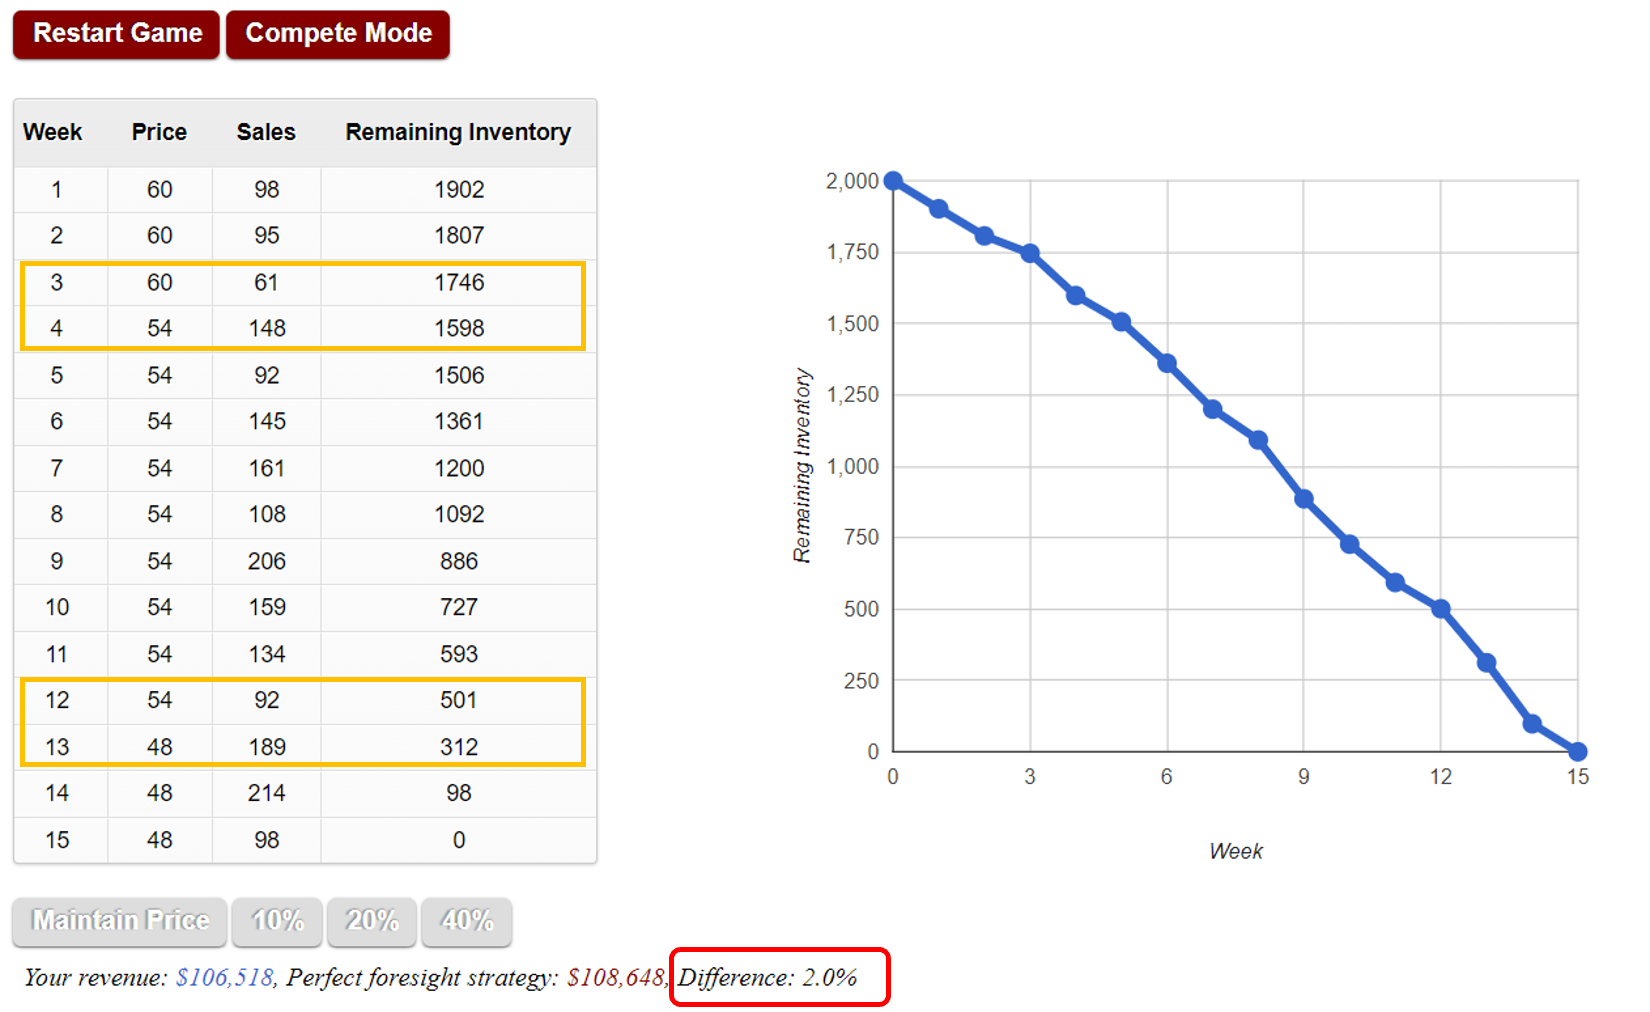
\includegraphics[width=0.75\textwidth]{pic/f1.png}
    \caption{Example of Markdown Strategy in the Retailer Game. \\\cite{RetailerGame}}
\end{figure}

\pagebreak
As a retailer, your objective is to maximize revenue, being as close as possible to the \emph{perfect foresight strategy} (i.e. with a \emph{difference} of 0\%). 
The optimized strategy or \emph{perfect foresight strategy} maximizes the revenue generated over the 15 weeks by implementing the right markdown strategy at the right time. 
Since the salvage value is \$0, the maximum revenue is mathematically equivalent to a linear sum of units sold at sale price for each sale price. 
The goal is to develop a data science approach to consistently minimize the difference between the expected revenue and perfect foresight strategy. 
We will use a sample of 15 “historical” sales, independent runs of the retail model and the web app to validate our strategies.

\section{Background}
The retail industry is increasingly focused on price markdowns to optimize profit, despite the challenges such as time constraints and sometimes the lack of historical data. 
Many revenue management models have tried to optimize the timing, duration and price discounts to influence consumer behaviour. 
Intuitively price drives demand. Markdowns of price increase reach and conversions to sales. 
Therefore, the optimal strategy balances maximizing revenue while minimizing the inventory left at the end of the sales. 
Any unsold inventory will likely contribute to environmental waste, incur disposal cost or increase inventory storage costs. 
In the last decades, innovations and new data management tools have allowed companies to move away from a manual pricing system and better manage their revenues.

\begin{figure}[h]
    \centering
    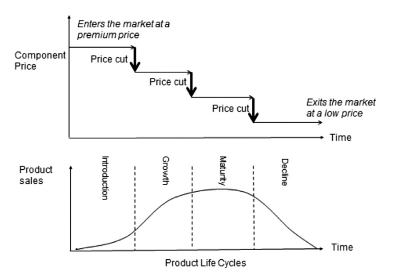
\includegraphics[width=0.5\textwidth]{pic/f2.png}
    \caption{Demand \& Price through Product Life Cycles. \\\cite{chung2015optimal}}
\end{figure}

Airline carriers started managing discounted fares back in the 1970s according to \linebreak 
\cite{talluri2004revenue}. 
The key pain point was optimizing sales through relevant discounted fares management. 
Statistical forecasting techniques and mathematical optimization methods have allowed airlines to frame their strategies, before extending other services such as hospitals, car rentals, cruise lines, railways, energy and broadcasting. 
In their paper, Talluri and van Ryzin highlight the importance and difficulty of modelling consumer behavior in predicting revenues. 
Some research discussed the implementation of dynamic pricing models and brought the problem back to a set of binary variables based on whether the customer will buy the article \cite{bitran1998structured,feng2000perishable,gallego1994optimal}. 
Talluri and van Ryzin focused on a choice-based approach that simulates consumer behaviour with a choice model by including probabilities of purchasing depending on the company’s offer panel, even without historical data.

On their side, fast-fashion retailers are looking at clearance price strategies before liquidation \cite{caro2012clearance}. 
In short, in retail, products are clustered by price categories; and each price category receives a clearance price. 
Therefore, the clearance price affects all the products from that price category. 
The approach then relies on dynamic programming. 
In 2008, the fast fashion multinational company Zara, opted to experiment with markdown strategies on multiple items. 
The model produced a 6\% or \$90M increase in sales revenue throughout the store and other cultural and business model improvements \cite{caro2012clearance}. 
The approach allows for a scalable, simple and reliable method to set pricing. 

\section{Proposed Strategies}
The literature on this web app pricing markdown structure suggest that revenue management is more complex than a one-size-fits-all approach. 
Several strategies or pricing policies may be appropriate for benchmarking and discovering an optimal or compromising strategy.
We will investigate several markdown and price change methods to understand their impact and potential application. 
We will evaluate the results using a simulation and web app validation. 
The simulation of the price and demand is done via a randomized sales distribution generated from mean price, standard deviation, and random number generation. 
Meanwhile the validation comes from a crosswalk code that interacts with the model and web app.

\subsection{Random Policy}
We will first investigate a random choice policy. 
This policy represents a likely worst-case scenario, where a company has no expertise and not logic to operate with. 
The policy will arbitrarily choose the pricing policy at each time t for future time periods.

Based on the random nature of the model and rules of the model, we expect a smaller distribution then the baseline mode (presented next). 
Since we cannot raise the price once lowered the cumulative probability of a 40\% discount approaches 40\% by the end of week 2 and 50\% by the end of the 15 weeks, which is the highest of any choice. 
Empirically we have observed that if the 40\% discount is offered early all units are sold within the 15-week period. 
The distribution of revenue should largely follow the distribution of the 40\% off price distribution we have observed.

\subsection{Baseline Model - Price Consistency}
The second strategy, we investigate a naïve approach to markdown strategies: do not change the price. 
We consider this a baseline policy as this is the easiest to follow and it does not require any price manipulation. 
While this policy ensures each item is sold at the highest price, it will likely leave unsold products. 
This naïve model is useful as a comparison point for the average revenue and standard deviation. 
In other words, the naïve “do nothing” model is a baseline to compare against and build off. 
The optimal price over the 15 weeks may be the original set price of \$60 or maybe some combination of price reductions, this model helps to determine the best approach in most situations.

We expect a highly varied revenue with a high standard deviation from this model that could be more consistent and optimal than the \emph{perfect foresight strategy}.

\subsection{Naïve Adaptive Likelihood Policy}
The next policy we investigate is a naïve adaptive likelihood method. 
This policy uses the previously observed data to predict the likelihood that given the current price the inventory will sell out. 
If at time t the inventory is not likely to sell out, the model investigates the remaining price choices and selects the first discount that gives a high probability of inventory sell out. 
For instance, at week 5 the model determines that the sales are not likely to lead to sell out, but the 10\% , 20\% and 40\% markdowns are all likely to lead to inventory sell out, so the model adjusts the \% off to 10\% to stimulate sales. 

\begin{figure}[h]
    \centering
    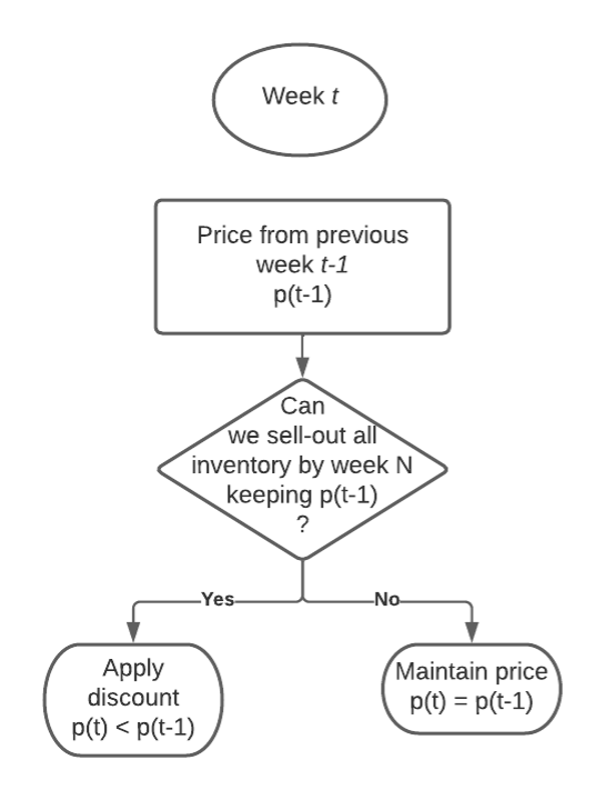
\includegraphics[width=0.5\textwidth]{pic/f3.png}
    \caption{Naïve Adaptative Likelihood Policy Decision Tree}
\end{figure}

\hfill \break
\indent We expect this model to have a high consistency of difference between revenue and the \emph{perfect foresight strategy}, with higher revenue than the baseline model and potential room for improvement.

\subsection{Adaptive Likelihood Price Policy}
The fourth policy is an adaptive likelihood price method. 
This method is similar to the naïve adaptive likelihood policy with a critical difference. 
Instead of using the estimated unit price increase this model aggregates the revenue from 10 separate forecasts for the remaining weeks. 
In other words, the model computes the expected revenue for 10 separate “what if” forecasts based on the observed distributions of historic data and assumes the price will not change before week 15.  
The revenue from the 10 forecasts run for each price point remaining at time t are summed and the one with the largest total revenue is used as the new price point. 
The model should help capture the original model’s randomness through more robust forecasts.

We expect this model to produce a more consistent difference between revenue and the \emph{perfect foresight strategy} with a higher average revenue than the naïve adaptive likelihood policy.

\subsection{Likelihood Demand Trend Projection}
The likelihood demand trend projection policy is an adaptive likelihood method that uses multiple runs of 15-week data to assume the same trends hold for future data. 
The given data suggests that each price reduction has a compounding effect on the unit volume sold. 
For instance, 10\% off increases unit sales by 30\%, and 20\% increases unit sales by 75\% compared to previous periods. 
The model uses rules based on the sales increase per price category to estimate the unit sales for the remaining periods. 
To accomplish this, the price distribution for the current model is added to the observed price distributions and the model evaluates the estimated likelihood of “out of stock condition”. 
In other words, if the estimated units sold by the end of the 15 weeks is less than the remaining units, the model increases the discount to stimulate the forecasted demand. 
Therefore, this approach is an improved version of the naïve adaptive likelihood method with additional assumptions on the demand’s behavior.

We expect this model to produce a more consistent difference between revenue and the \emph{perfect foresight strategy} with a higher average revenue than the naïve adaptive likelihood policy.

\subsection{Short-term Moving Average Naïve}
Next, we investigate a naive moving average approach. 
In this approach the previous 3-day demand is accumulated into a moving average to forecast demand for time t+1. 
The 3-day average helps smooth any randomness in the demand curve due to noise. 
The function considers the momentum of previous 3 week of sales to determine if the current trajectory of sales will result in no inventory at the end of the 15-week period. 
If the sales momentum from the previous 3 days is lower than the average number of units needed to sell out by the end of the period, the price is dropped. 

\begin{figure}[h]
    \centering
    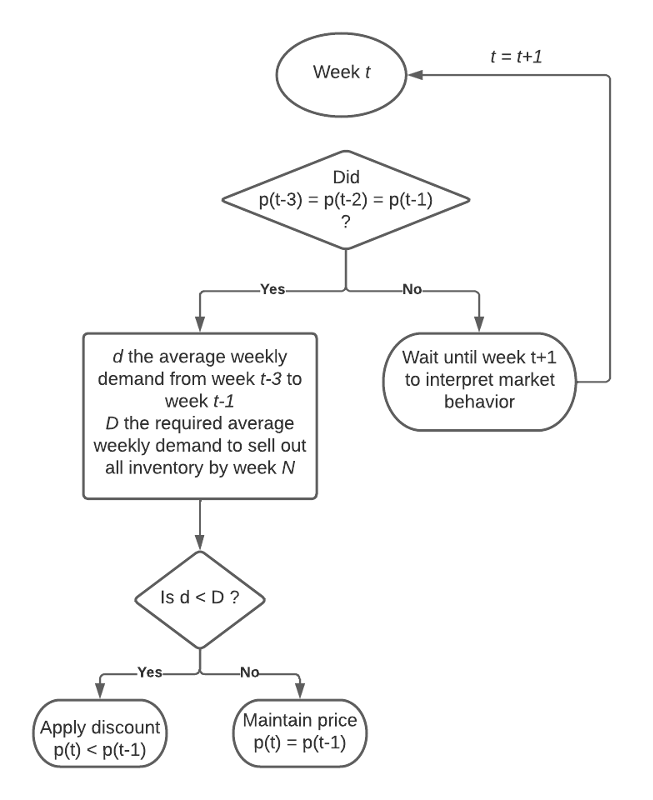
\includegraphics[width=0.5\textwidth]{pic/f4.png}
    \caption{Naïve Adaptative Likelihood Policy Decision Tree}
\end{figure}

Let’s consider an example: at week 4, the previous 3 weeks sales average is 100 units per week. There are 1,700 units left. 
The average sales needed to sell out of inventory is 141 units (1,700 units / 12 weeks). 
Since the moving average sales (100 per week) is below the required 141 sales per week the model will lower the price. 
The model will then wait 3 weeks to allow the new policy to take shape before re-examining a price decrease. 
The same factors will help decide whether to lower the price again or not. 
This simple model accounts for the randomness of demand and helps ensure more sales by valuing sales momentum over optimal price strategy.

We expect this model to have a higher consistency than the baseline mode, lower the price quickly to the lowest amount and consistently sell out of all units.  
This model is likely better than the baseline but could be better as the price has a maximum decrease speed.

\subsection{Long-term Adaptive Moving Average with Wait}
The final policy we will investigate is an adaptive moving average with a policy. 
This policy is similar to the naïve moving average policy with added levels of complexity. 
The moving average is used to predict the total sales over the remaining time and compares it to the remaining amount. 
If the predicted sales (in units) for the future periods is lower than the total remaining units in inventory, then the price will decrease in an effort to increase sales. 
Unlike the previous methods, this strategy helps smooth out the randomness in the data more so than the previous short term moving average policy. 

We expect this model to have a lower difference consistency than the short-term naïve average, since it is likely that more of the units sold will reach different price points faster than the short-term average model. 
However, we also expect this model to have the highest average revenue of all models.

\subsection{Reinforcement Learning}
A proposed final future state policy is the reinforcement learning strategy. 
Artificial intelligence models rely on supervised reinforcement learning which learn as they go. 
The models are rewarded for certain actions and attempt to maximize the reward, relying on previous runs or iterations to build off of. 
These models are ideal for repeated tasks that have defined conditions. For example, Open AI in 2019 demonstrated a reinforcement learning model that simulated a game of hide and seek \cite{baker2019emergent}. 
We will apply reinforcement learning to this problem, where the reward function is the maximization of the revenue, and the inputs are from the app itself. 
While this model offers little explanation ability since reinforcement learning models are black box models, the reinforcement learning policy may perform better than previous policies.

We expect that the reinforcement learning model will have the highest revenue and the lowest revenue distribution of all models previously tested.

\section{Implementation}

\subsection{Data Treatment}
While we have access to 15 runs of “historical” data, before using this data, we must apply data preprocessing.

First, we must ensure that the data does not contain errors or null values. 
We, therefore, removed null rows and appended the run number (1-15) to each observation within the data. 
After the data cleanup, we are left with a dataset containing the run number, the week number, the price of the item (\$60, \$54, \$48, \$36), the unit demand and the revenue generated from that week of sales.

Second, we need to transform the data into more meaningful formats. We grouped the data by price to measure unit sales’ standard deviation and mean. This first grouping was helpful in the naïve price policy we applied. 
We also grouped the data by price to measure the mean and standard deviation of the unit sales compared to the previous week. In other words, what is the \% increase (or decrease) in unit sales when a new price point is set. 
It may be that a 20\% decrease in price increases unit sales by 70\%, independent of the previous price point.

Based on some casual observations of the data, the distributions appear roughly normally distributed, we will use this as a basis for simulation and modelling.

\subsection{Simulation}
To forecast the impact of the pricing strategies we are investigating, we must test the policies against data. 
Since we cannot access the exact equation or similar random number generator used for the web app, we must first utilize simulations. 
The model built takes the policy, the average and the standard deviation of the observed price points and generates 100 simulations. 
For each simulation and each time t, the model generates unit sales based on a numpy random normal method using the mean and standard deviation of the current price point. 
The simulation approach best reflects a real-life scenario as a forecast function is generally unknown, resulting in a reliance on past data to predict future demand. 
The generated numbers reflect the data distribution found within the historical data.

\begin{itemize}[leftmargin=*]
    \item Pseudo Code of Simulation Approach and Validation
\end{itemize}

\begin{algorithmic}[1]
    \Procedure{Policy}{$list\ of\ sales,\ list\ of\ price$}
        \State \textbf{generate} price for the next period \textbf{with} current run sales and prices
        \State \textbf{return} price
    \EndProcedure
    \State
    \Procedure{Simulate}{$policy,\ means\ per\ price, stdevs\ per\ price$}
        \For{t = 1 to 15}
            \State \textbf{generate} unit sales \textbf{with} mean, stdev, and current price
            \State \textbf{generate} price \textbf{for} next period \textbf{with} given policy
        \EndFor
        \State \textbf{return} revenue
    \EndProcedure 
    \State
    \For{policy \textbf{in} policy candidate list}
        \For{t = 1 to 100}
            \State \textbf{generate} means per price, stdevs per price \textbf{for} current simulation run 
            \State policy results = $Simulate$ (policy, means per price, stdevs per price) 
            \State \textbf{save} policy results
        \EndFor
    \EndFor
\end{algorithmic}

\subsection{Validation}
The simulation approach helps validate the models and quickly select the best policy with limited information. 
However, for this context, we need not rely solely on the simulation data, we can instead use the actual data from the web app. 
The assumptions and approach we have previously laid out may have unknown challenges or other pitfalls. 
In this scenario we are not limited to the simulation and approximation of “real world data”. 
We will therefore validate the simulation results using the web application. 
To implement the validation, we will utilize a selenium-based python script which goes between the code and user interface on the web app. 
Each policy is tested in real-time against the app while recording the results to evaluate after the fact. 

\begin{itemize}[leftmargin=*]
    \item Pseudo Code of Policy Validation using WebApp
\end{itemize}

\begin{algorithmic}[1]
    \Procedure{Policy Validate}{$policy$}
    \State URL = "http://www.randhawa.us/games/retailer/nyu.html"
    \For{ t= 1 to 15}
        \State \textbf{retrieve} unit sales \textbf{from} website
        \State \textbf{generate} price \textbf{for} next period \textbf{with} given policy
    \EndFor
    \State \textbf{return} expected return
    \EndProcedure
    \State
    \For{policy in policy candidate list}
        \For{t = 1 to 100}
            \State policy results = $Policy\ Validate$ (policy) 
        \EndFor
    \EndFor
    \State \textbf{plot} policy results
\end{algorithmic}

\section{Discussion and Recommendations}

\subsection{Policy Comparison}
In this report, we proposed eight different pricing strategies including heuristic, probability-based, traditional moving average, and reinforcement learning approaches. 
All except the reinforcement learning approach were simulated and validated on the web app. 
Based on the simulation results in Figure 5, Naïve Adaptive Likelihood Policy provides the highest average revenue followed by likelihood shared.

Figure 5 demonstrates the relationship between prices and sales in different policies. 
Policies with better performance such as Naïve Adaptive Likelihood, Likelihood Demand Trend Projection, and Moving Average Naïve, share a common characteristic: adopting price change steadily. 
These models take more time waiting and observing the market before adjusting prices accordingly. 
Conversely, Long Term Adaptive Moving Average and Adaptive likelihood price policy tend to lower the price immediately once the product is not in great demand. 
These policies often drop prices around week 6 to week 8 and significantly increase sales afterward. 
Yet, with discounted prices, the average revenue does not outperform others. 
Figure 6 demonstrates the weekly sales figures for each model and validates this observation. 
For instance, the average long-term policy drops the price around the 8th week for an immediate sales increase, but quickly panics and keeps lowering the price until the 40\% discount is reached. 
The models with a slower price markdown strategy perform best in total revenue generation.

In addition to the maximization of revenue, model consistency is another key aspect of the models. 
Suggesting a markdown strategy with a high level of variability will likely create more issues than it solves.  
Figures 7 and 8 demonstrate the model predictions’ consistency or lack thereof.  
In Figure 9, the most consistent strategy is the random choice policy. 
The conditional probability of selecting 40\% within the first 2 turns is 43\% based on the rules of the web app which prevent prices from changing once the 40\% discount is given. 
The randomness model generates an average of \$80k, much lower than all other models except the baseline. 
The baseline model, meanwhile, has a broad range of revenue values, as seen by the value of the IQR, which is approximately \$20k. 
This is likely a direct reflection of the randomness introduced into the model to simulate demand. 
All other models have a lower range of values and, thus, are more consistent than the baseline policy. 
The likelihood price policy demonstrates the best consistency of values with an IQR of approximately \$10k. 
Therefore 50\% of all models run with this policy will have a revenue of \$73-\$83k.  
Consistency of revenue prediction is equally important to the total revenue.

Each model and policy have their own logic and results. 
The baseline and random functions offer little in consistency or maximizing revenue, respectively. 
These two models represent the two extremes of the desired model characteristics that maximize revenue and minimize spread. 
Neither characteristic alone appears sufficiently robust to recommend as a strategy with a retail firm. 
All other models offer a more nuanced approach to balancing the revenue and spread. 
The remaining policies can be grouped into either a slow change in sale price or a quick change in sale price. 
The slower-moving sales balance revenue generation and distribution after 15 weeks. 
Finally, we recommend a policy based on those presented above.\\

\begin{figure}[h]
    \centering
    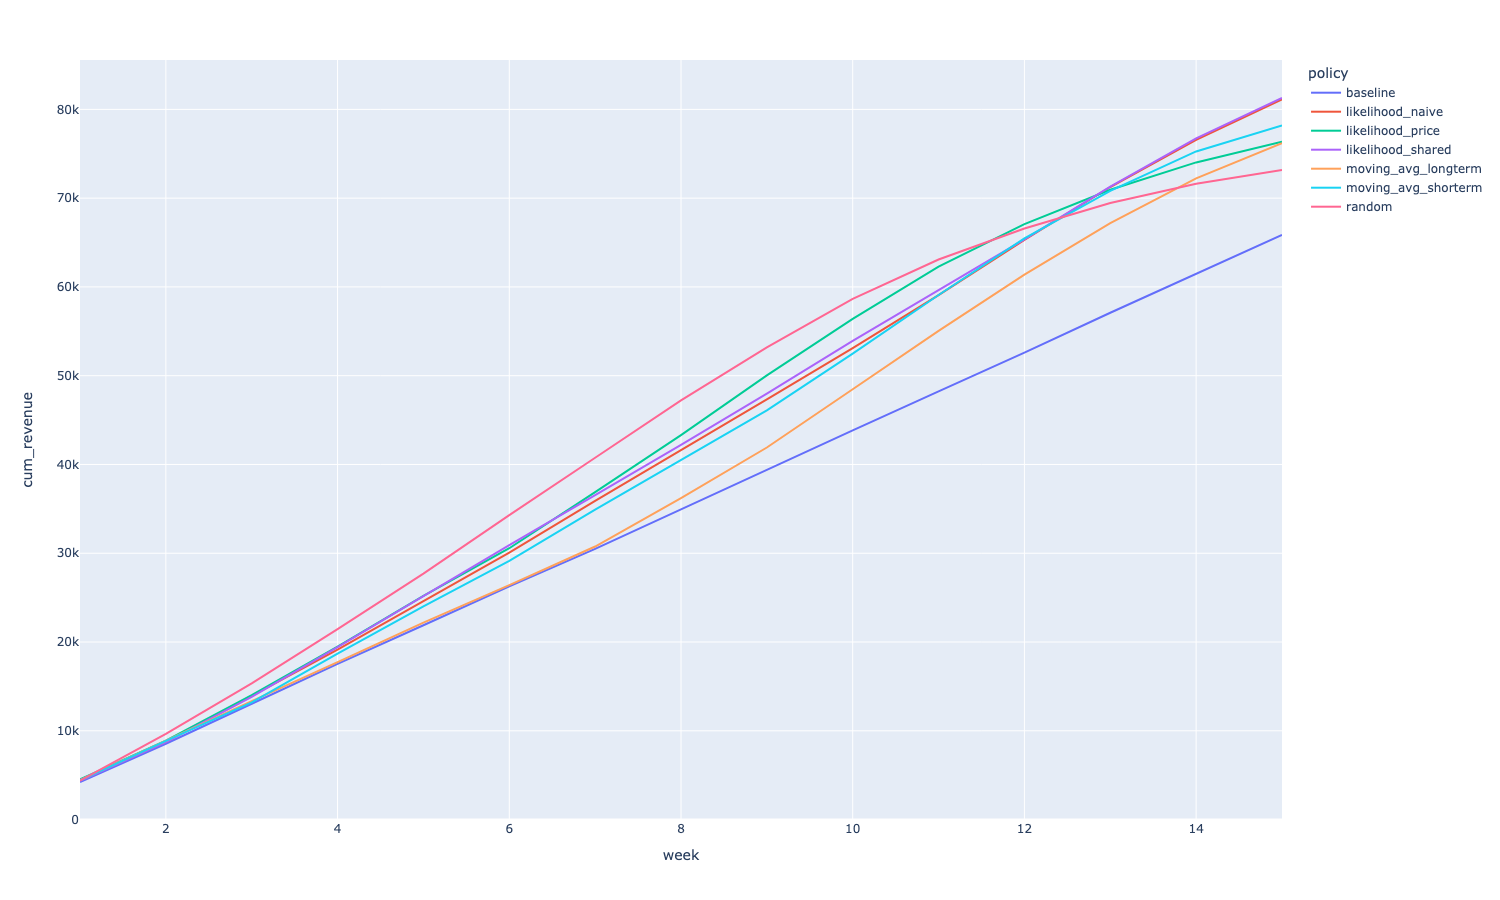
\includegraphics[width=0.75\textwidth]{pic/f5.png}
    \caption{Average Cumulative Revenue by Policy and Week}
\end{figure}

\begin{figure}[h]
    \centering
    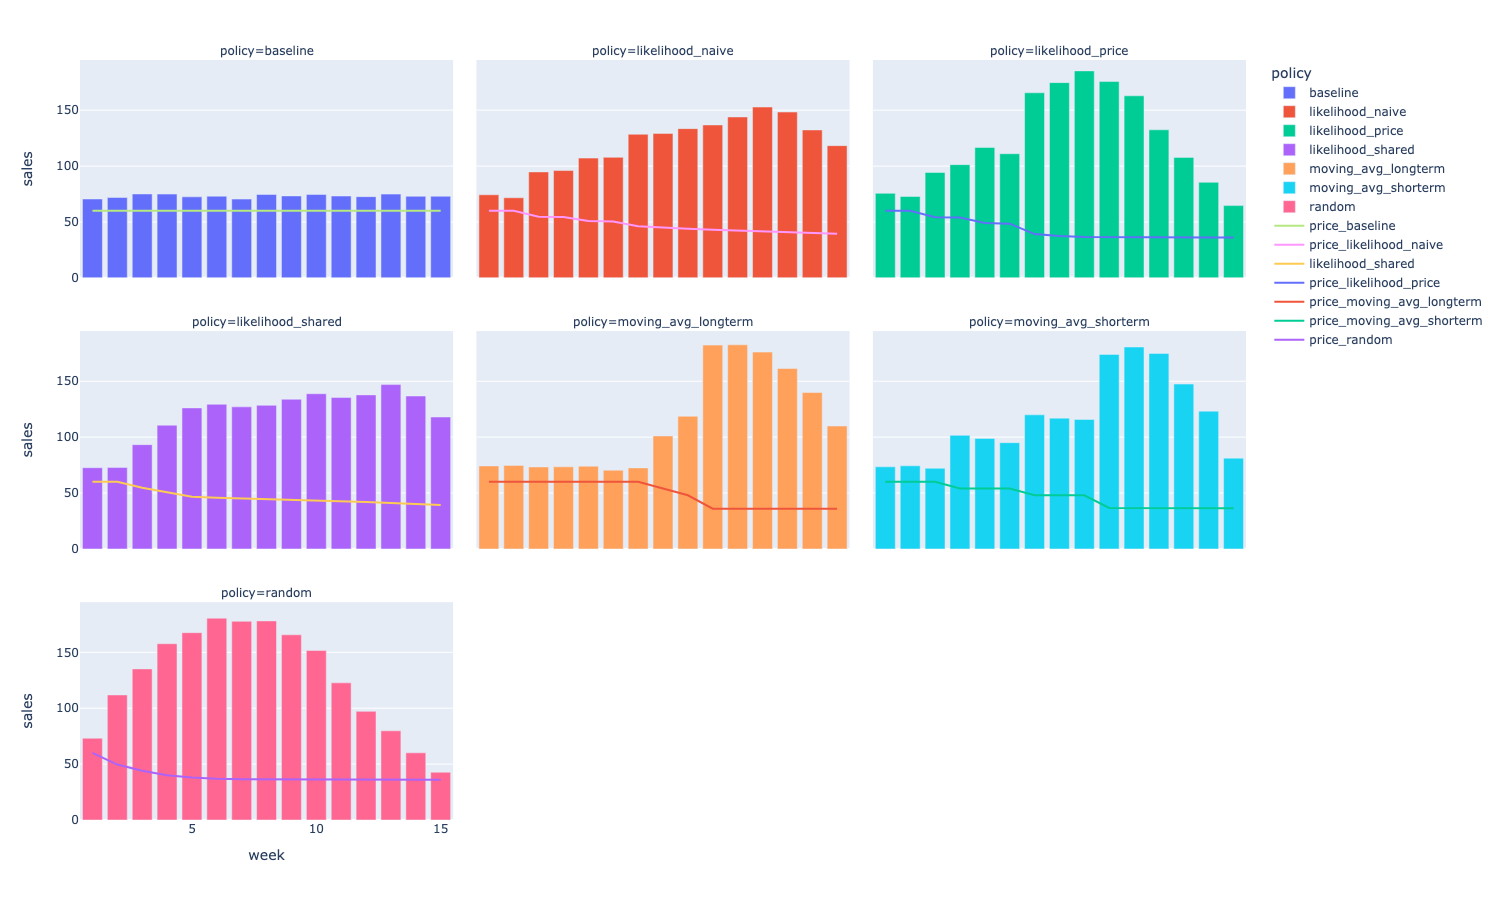
\includegraphics[width=0.75\textwidth]{pic/f6.png}
    \caption{Average Weekly Revenue by Policy, and Week with Line of Unit Prices}
\end{figure}
\pagebreak
\hfill \break
\begin{figure}[h]
    \centering
    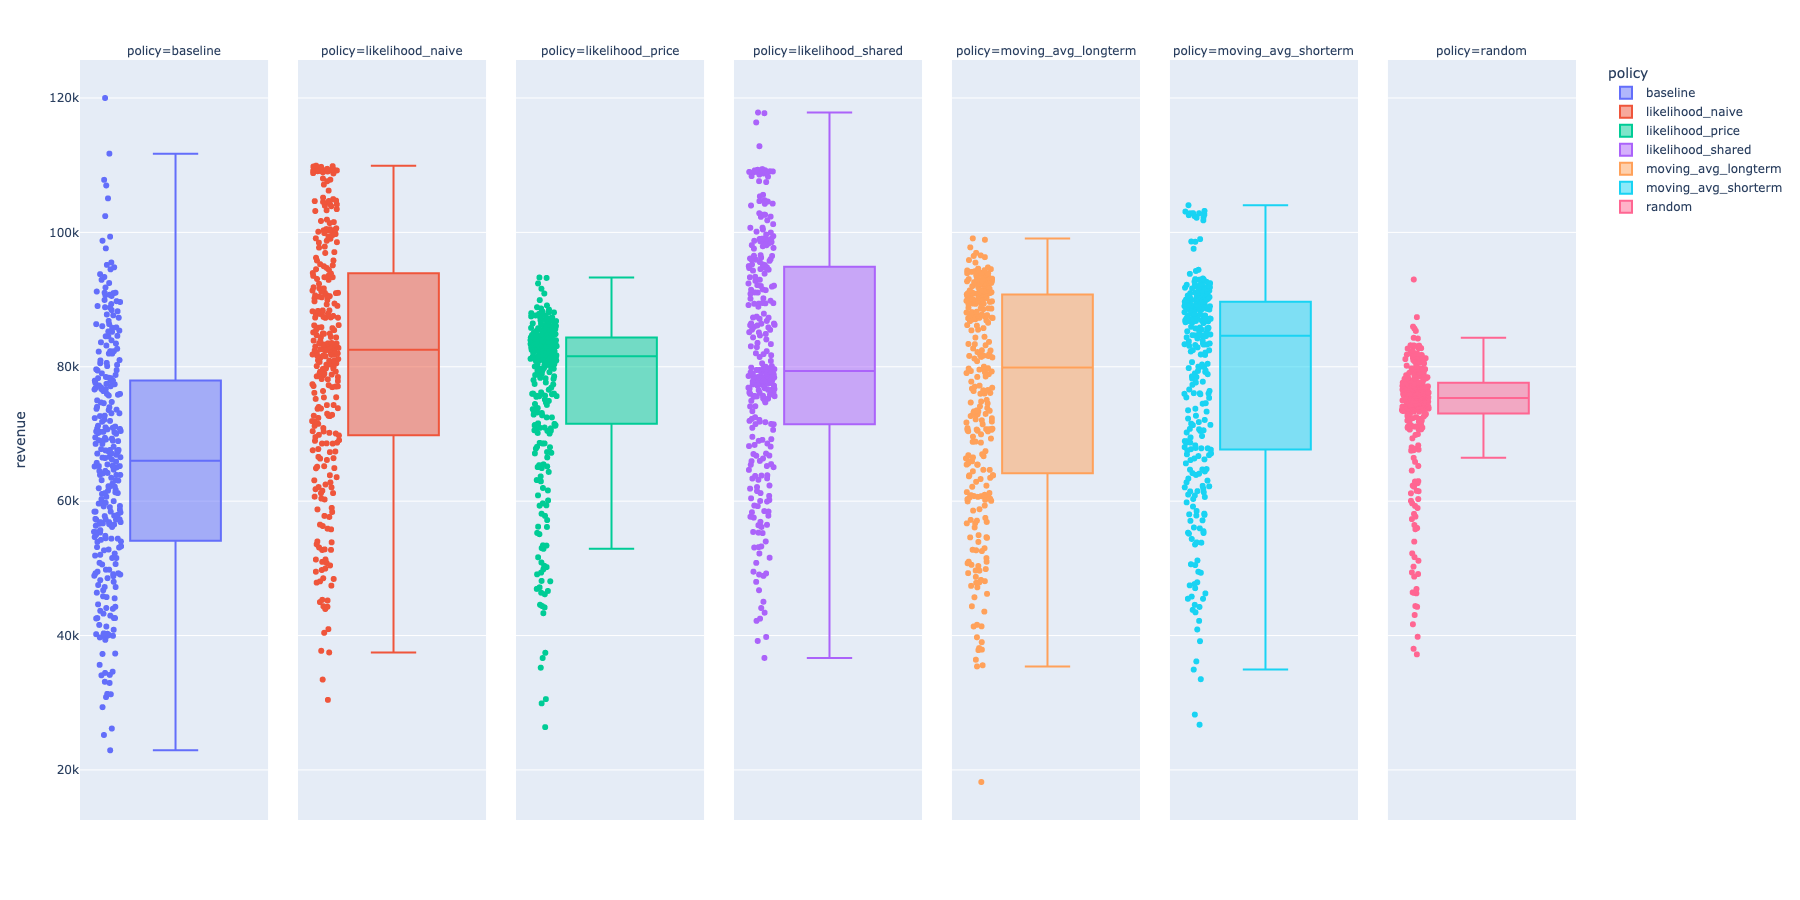
\includegraphics[width=0.75\textwidth]{pic/f7.png}
    \caption{Whisker Plot per Policy based on Revenue Distribution from 100 Simulated Runs. Note: Optimal Revenue for the run depends on Random Seed but is approximately \$100k}
\end{figure}
\hfill \break
\begin{figure}[h]
    \centering
    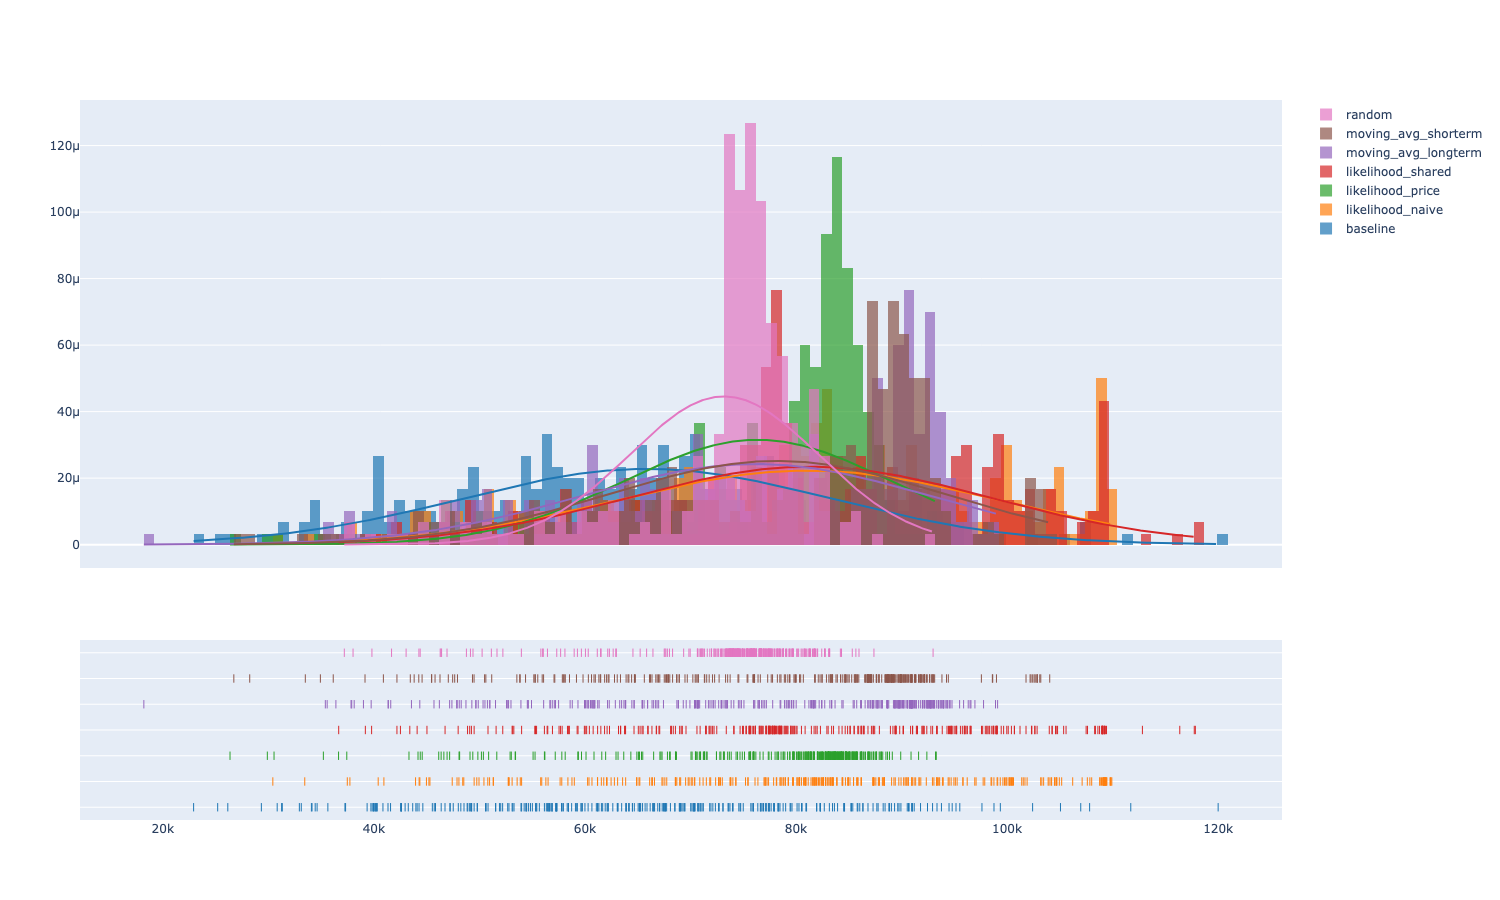
\includegraphics[width=0.75\textwidth]{pic/f8.png}
    \caption{Combination of Bar Chart with approximated Normal Distribution overlay and Rug Chart for Distribution of Simulated Revenue based on Policy}
\end{figure}

\pagebreak
\subsection{Recommended Policy}
Based on the comparison and results from validation, we recommend adopting the likelihood naïve policy. 
As figure 8 illustrates, once the policies are validated using the web app the likelihood naïve policy best balances the high revenue, with a median of \$95K and an IQR or \$15K. 
The next best policy, the Likelihood Demand Trend Projection or colloquially known as the likelihood shared model has a median of \$100k but an IQR of \$20k. 
Between the two best models observed the naïve likelihood policy produces consistently higher returns than the other strategies. Furthermore, based on Figure 10 the naïve likelihood model minimizes the difference between the perfect strategy with a medial of 2.5\% difference. 

There is no perfect approach to modeling a fashion retailer’s markdown strategy. The underlying functions and randomness of the real world are too difficult for even the best simulations. 
However, using data science and a trial-and-error approach we can conclude that of the tested models, the best approach to approximating fashion retailer’s markdown strategy is a naïve pricing model where the price distribution is the most likely to lead to inventory sell out. 
\pagebreak
\hfill \break
\hfill \break

\begin{figure}[h]
    \centering
    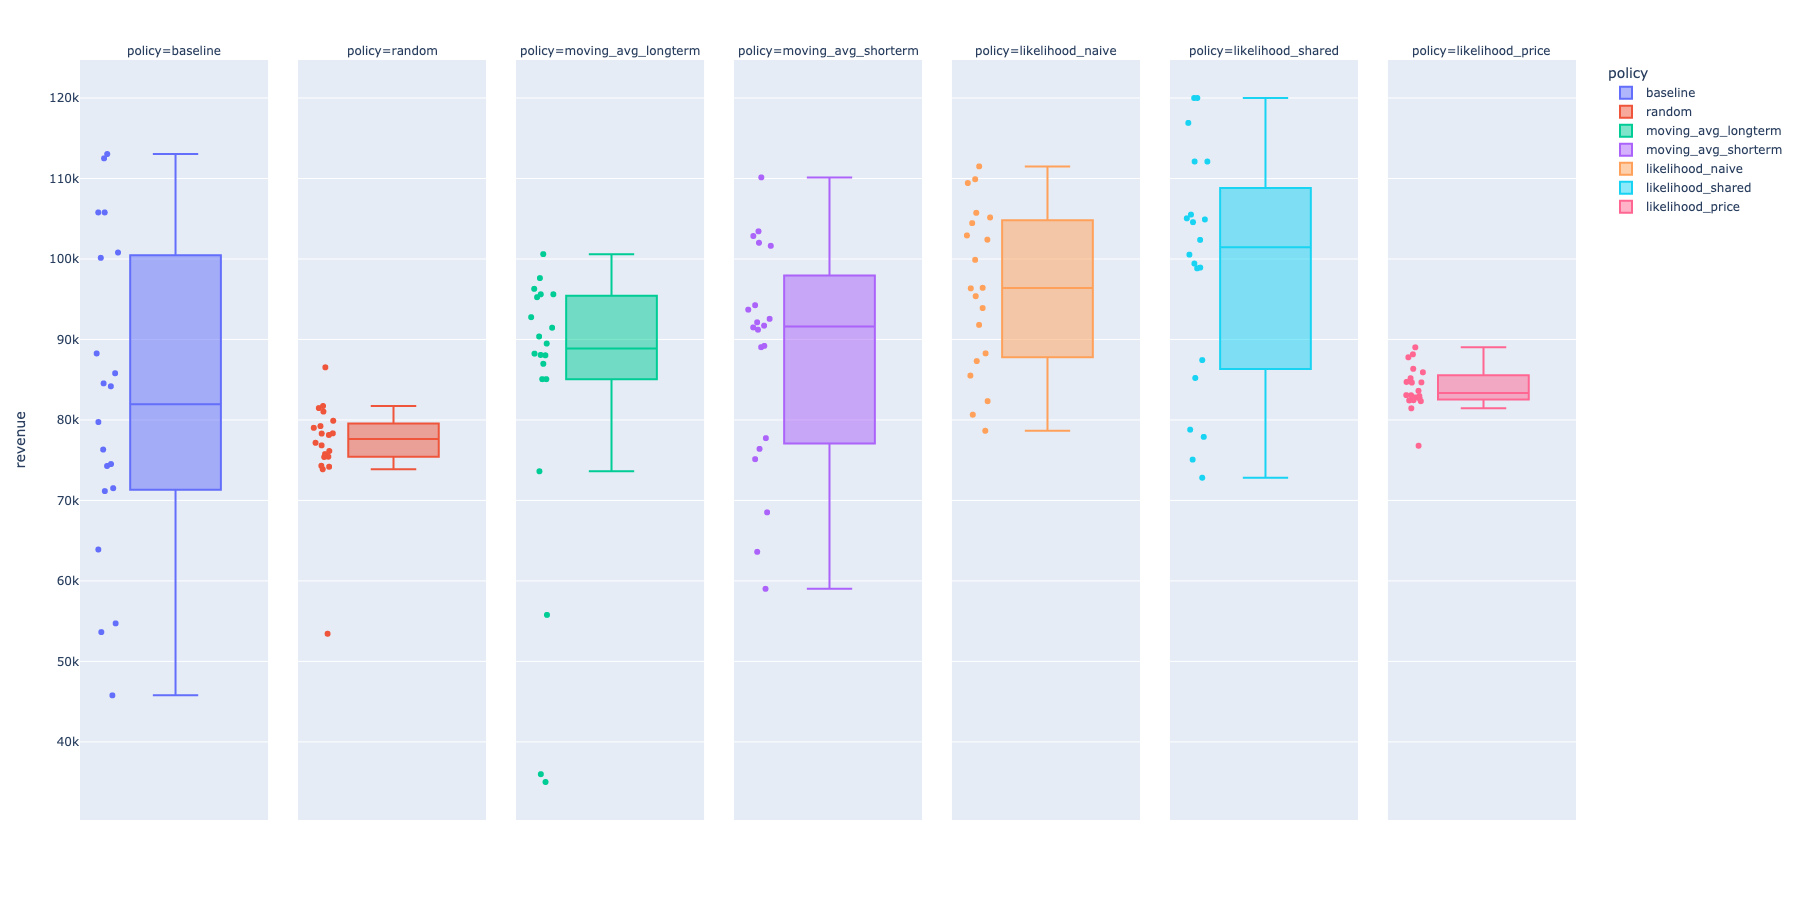
\includegraphics[width=0.95\textwidth]{pic/f9.png}
    \caption{Validation: Revenue Distribution}
\end{figure}
\hfill \break
\begin{figure}[h]
    \centering
    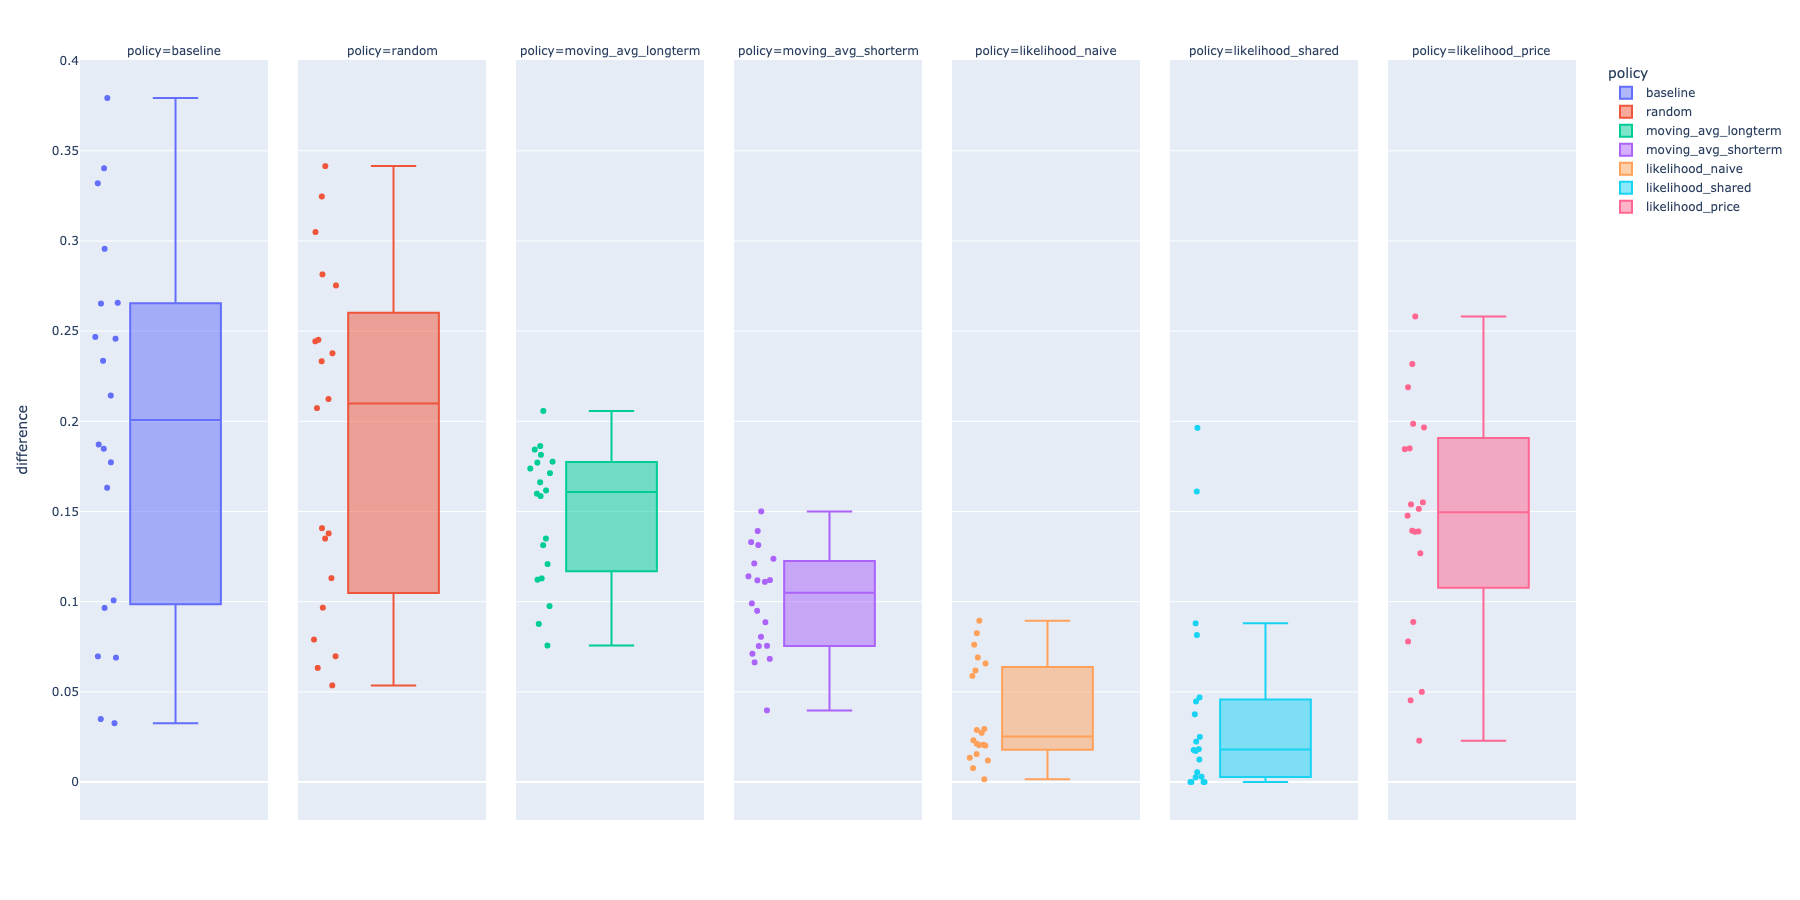
\includegraphics[width=0.95\textwidth]{pic/f10.png}
    \caption{Validation: Difference Distribution}
\end{figure}

\pagebreak
\bibliographystyle{apalike}
\bibliography{ref.bib}

\end{document}